\documentclass[conference,a4paper,twoside]{IEEEtran}
\RequirePackage[T1]{fontenc}
\usepackage[utf8x]{inputenc}
\usepackage{lmodern}
\usepackage{cite}
\usepackage[ngerman]{babel}
\usepackage{amsmath,amssymb,amsfonts}
\usepackage{graphicx}
\usepackage{textcomp}
\usepackage{xcolor}
\usepackage{url}
\usepackage{float}
\usepackage{svg}
\def\BibTeX{{\rm B\kern-.05em{\sc i\kern-.025em b}\kern-.08em
    T\kern-.1667em\lower.7ex\hbox{E}\kern-.125emX}}
\begin{document}

\title{FEM-Hausarbeit: Automatisierung der Berechnung}

\author{
  \IEEEauthorblockN{Johannes Frielingsdorf}
  \IEEEauthorblockA{\textit{Fakultät für Informations-, Medien- und Elektrotechnik} \\
  \textit{Technische Hochschule Köln}\\
  Köln, Deutschland \\
  johannes.frielingsdorf@th-koeln.de}
}

\maketitle

%Polygone Afg. 1: 19642 nodes 32928 elements
%Polygone Afg. 2: 22162 nodes 37168 elements
%Polygone Afg. 3:

\section{Einführung}
In diesem Projekt wurde die Python Scripting-Schnittstelle von Agros2D verwendet, um systematisch Änderungen in der Simulationsgeometrie aus dem vorherigen Projekt des "Magnetischen Kreises" zu untersuchen.

Alle Simulationsdateien werden aufgabenweise als .zip-Archiv abgegeben, da im Rahmen der Projektbearbeitung mehrere Dateien pro Aufgabenstellung erstellt wurden. Dies umfasst sowohl mehrere Python-Skriptdateien, da in der Regel die Erstellung der Simulationsumgebung in eine eigene Datei ausgelagert wurde.

Da unter Ubuntu 20.04 offenbar matplotlib in Agros2D nicht verfügbar ist und auch eine Nachinstallation nicht gelang, wurde abweichend von der Aufgabenstellung jeweils eine .csv-Datei mit den Simulationsergebnissen durch Agros2D angelegt, die anschließend mit Gnuplot visualisiert wurde. Daher befindet sich in den jeweiligen Projektordnern eine .gnuplot-Datei zur Konfiguration des Plots, sowie Shellskripte zum Aufruf von Agros2D mit dem Python-Skript sowie Gnuplot.

Weiterhin steht das das Git-Repository des Projektes unter \url{https://github.com/bazjo/Agros2D-Automation} zur Verfügung.

\section{Aufgabenstellung 1}
In der ersten Aufgabenstellung wird der Elektromagnet aus Projekt 2 ohne Permanentmagnet erneut betrachtet. Es wird die magnetische Flussdichte im Luftspalt sowie die Anziehungskraft auf das I-Joch für verschiedene Feldstärken untersucht. Dazu wird eine Funktion zur Generierung einer halbseitigen Simulationsgeometrie unter Ausnutzung der Spiegelsymmetrie erstellt. Eine Simulation wird jeweils für Ströme von $1\ A$ bis $64\ A$ in $1\ A$-Schritten durchgeführt.

Dargestellt ist beispeilhaft eine Stromstärke von $64\ A$. Abb.~\ref{assignment_1_geometry} zeigt die Simulationsgeometrie, Abb.~\ref{assignment_1_mesh} das generierte Netz und Abb.~\ref{assignment_1_simulation} die resultierende Flussdichteverteilung. Die Netzknotenanzahl betrug in diesem Fall 19642; die Anzahl der Polygone 32928.

\begin{figure}
\centerline{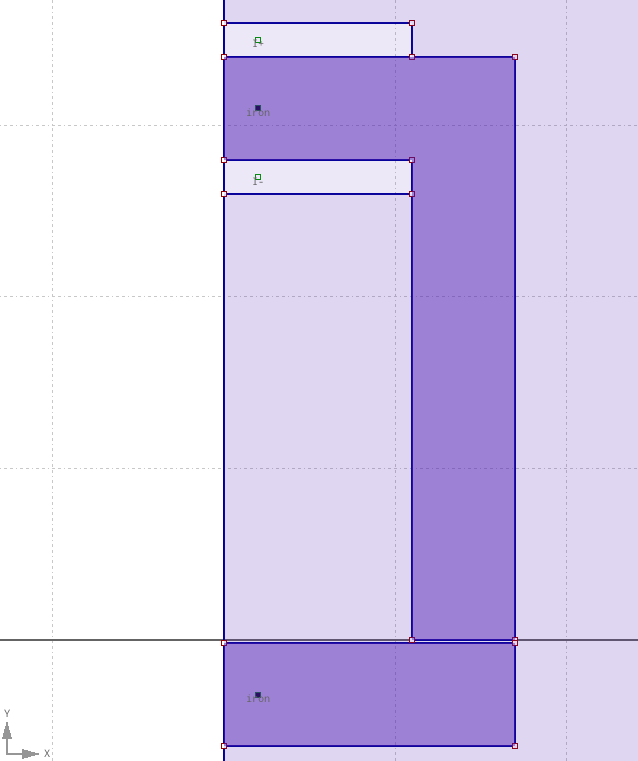
\includegraphics[width=0.7\columnwidth]{../assets/assignment_1_geometry.png}}
\caption{Simulationsgeometrie in der ersten Aufgabenstellung; $I = 64\ A$.}
\label{assignment_1_geometry}
\end{figure}

\begin{figure}
\centerline{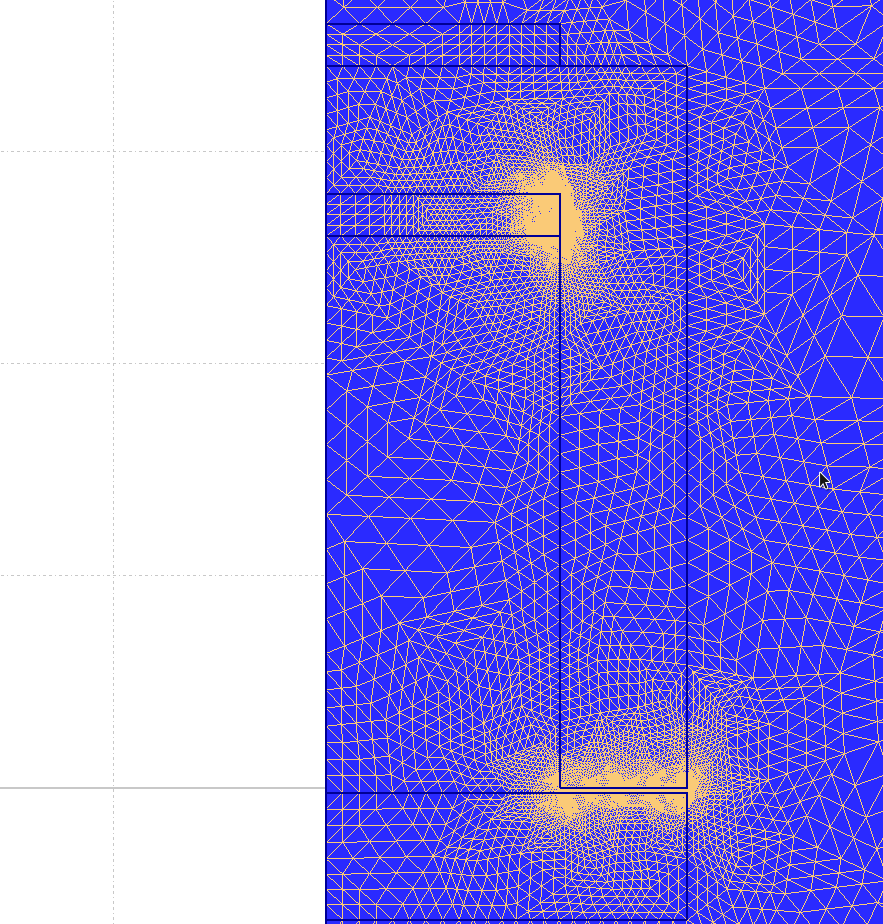
\includegraphics[width=0.7\columnwidth]{../assets/assignment_1_mesh.png}}
\caption{Simulationsvermaschung in der ersten Aufgabenstellung; $I = 64\ A$.}
\label{assignment_1_mesh}
\end{figure}

\begin{figure}
\centerline{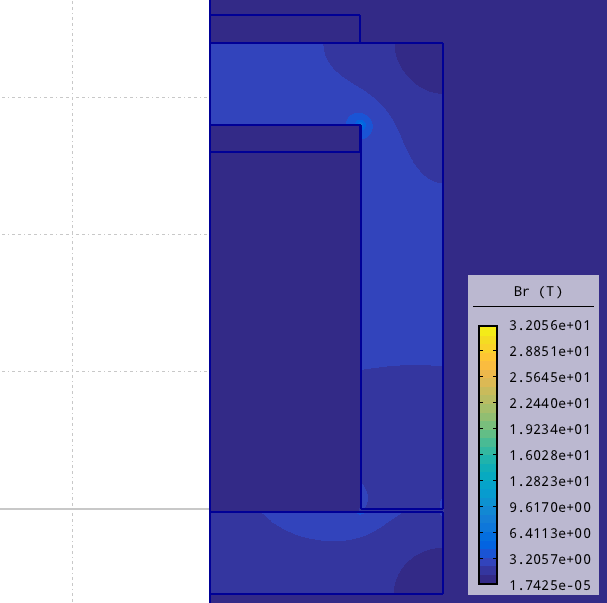
\includegraphics[width=0.7\columnwidth]{../assets/assignment_1_simulation.png}}
\caption{Flussdichteverteilung in der ersten Aufgabenstellung; $I = 64\ A$.}
\label{assignment_1_simulation}
\end{figure}

\begin{figure}
\centerline{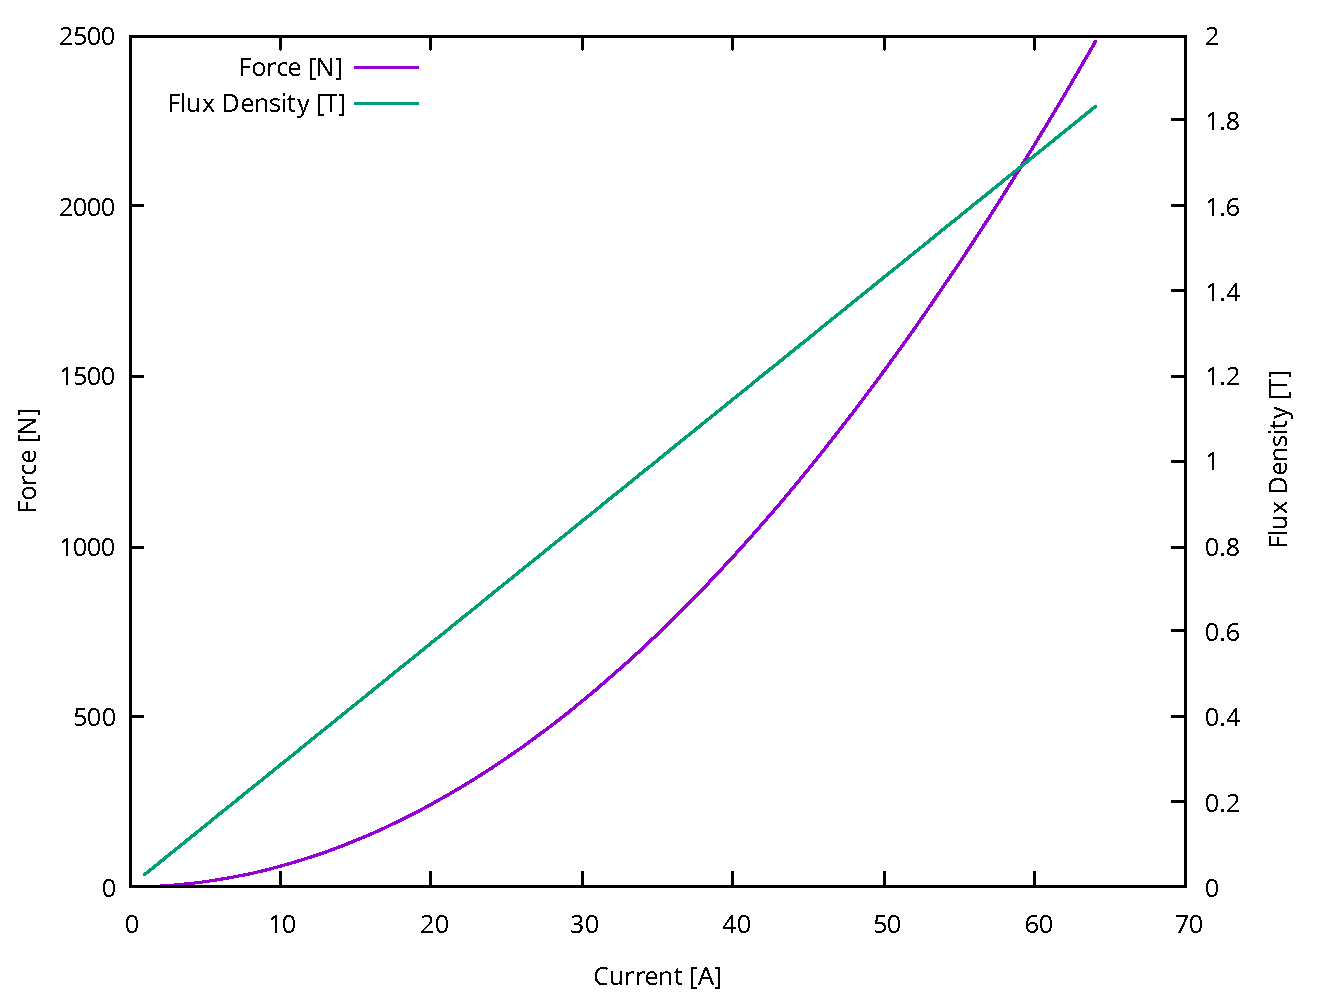
\includegraphics[width=\columnwidth]{../assets/assignment_1_plot.pdf}}
\caption{Flussdichteverteilung in der ersten Aufgabenstellung; $I = 64\ A$.}
\label{assignment_1_plot}
\end{figure}

In dieser und in allen folgenden Aufgaben wurde stets, wo nicht anders angegeben, ein Verfeinerungsniveau und die Polynomordnung 2 verwendet.

\end{document}
